\chapter{Hitting Times and Learning the Gap}\label{ch:hitting}\index{hitting time}\index{moderate deviations}\index{hazard rate}

A gap is a rate, and probability has more than one way to read a rate. The correlator reads it from the decay of a covariance, and Chapter~\ref{ch:kac} read it from the mixing of a Markov chain. This chapter records two further readings: the hazard rate of a hitting time, in the manner of Roberts and Shortland \cite{RS95,RS97}, and the scale of fluctuations between the central limit theorem and large deviations, in the manner of Rubin and Sethuraman \cite{RuSe65}. The hazard rate gives a theorem about the gap and an estimator. The moderate deviation scale gives honest sample sizes and, under a hypothesis we state, a necessary test for a unique vacuum. Neither proves the gap in four dimensions. We say where each helps.

The second part of the chapter turns from what the gap is to how it is learned. Section~\ref{ch:plgbc} develops sufficient statistics of a lattice gauge field, particle learning \cite{CJLP} and generative Bayesian computation \cite{PSgbc}, which learns the map from statistics to parameters from simulations, and asks whether they are useful for the mass gap. Section~\ref{ch:quantum} asks what quantum computation could add \cite{PSX23}. The chapter closes Part II: apart from the theorems proved for one group variable and one plaquette, everything in it is an estimator, a restatement or a numerical experiment.

\section{The hazard rate of a hitting time}\index{Roberts, G. O.}\index{Shortland, C. F.}

Roberts and Shortland studied the first time a diffusion hits a boundary through its hazard rate $r(t)=-\frac{d}{dt}\log P(T>t)$, approximated it by tangent boundaries, and used the result to price barrier options with time dependent coefficients. The object that matters for us is the limit of the hazard rate. For a reversible diffusion with generator $L$ and invariant probability $\mu$, and a closed set $A$ with $\mu(A)>0$, let
\[
\lambda_D(A)=\inf\Big\{\frac{\mathcal E(f,f)}{\mu(f^2)}:\ f=0\ \text{on}\ A\Big\},\qquad \mathcal E(f,f)=\mu\big(f(-L)f\big),
\]
be the bottom of the spectrum with Dirichlet condition on $A$. When $\lambda_D(A)$ is an isolated eigenvalue, as on a compact state space, $P_\nu(T_A>t)$ decays like $e^{-\lambda_D(A)t}$ for every starting law $\nu$ with a square integrable density that charges the ground state, and the hazard rate of $T_A$ tends to $\lambda_D(A)$. The gap $\lambda_1$ is the bottom of the spectrum on functions of mean zero.

\begin{theorem}[Hitting times bracket the gap]\label{thm:hitgap}\index{Dirichlet eigenvalue}
For a reversible diffusion with invariant probability $\mu$ and gap $\lambda_1$:
\begin{enumerate}
\item[(i)] for every closed set $A$ with $\mu(A)>0$, $\lambda_1\le\lambda_D(A)/\mu(A)$;
\item[(ii)] $\lambda_1\ge\inf\{\lambda_D(A):\mu(A)\ge\frac12\}$.
\end{enumerate}
Hence, writing $r_*$ for the infimum in (ii), $r_*\le\lambda_1\le2r_*$: the gap is positive if and only if $\lambda_D(A)$ is bounded away from zero over the closed sets of measure at least one half; on a compact state space $\lambda_D(A)$ is the limiting hazard rate of $T_A$.
\end{theorem}

\begin{proof}
(i) If $f$ vanishes on $A$ then by the Schwarz inequality $\mu(f)^2\le\mu(f^2)\,\mu(A^c)$, so $\operatorname{Var}_\mu(f)\ge\mu(A)\,\mu(f^2)$, and the Poincar\'e inequality gives $\mathcal E(f,f)\ge\lambda_1\mu(A)\mu(f^2)$. (ii) Let $f$ be in the domain of the form, let $m$ be a median of $f$, and put $f_\pm=(f-m)_\pm$. Each of $f_+$ and $f_-$ vanishes on a set of measure at least one half, so $\mu(f_\pm^2)\le\mathcal E(f_\pm,f_\pm)/r_*$ by the definition of $r_*$. The form of a diffusion is local, $\mathcal E(f_+,f_-)=0$, so $\mathcal E(f_+,f_+)+\mathcal E(f_-,f_-)=\mathcal E(f,f)$. Hence $\operatorname{Var}_\mu(f)\le\mu\big((f-m)^2\big)=\mu(f_+^2)+\mu(f_-^2)\le\mathcal E(f,f)/r_*$, which is $\lambda_1\ge r_*$; no eigenfunction is needed, so it does not matter whether the gap is attained. The last statement takes $\mu(A)\ge\frac12$ in (i).
\end{proof}

Both halves are standard for Markov chains, beside Cheeger's inequality; we have not seen them used for the mass gap. The change of object is the point. A correlator is a signed quantity whose signal to noise ratio falls exponentially in time; a survival probability is positive, and the maximum likelihood estimate of a constant hazard is a ratio of sufficient statistics, the number of exits divided by the total time at risk.

When there is a reflection, the factor of two disappears.

\begin{proposition}[Reflection]\label{prop:hitreflect}\index{reflection positivity}
Let $\rho$ be an involution of the state space that preserves $\mu$ and commutes with $L$, and suppose that the complement of its fixed set $F$ has exactly two components, each connected and exchanged by $\rho$, so that every continuous path from a point to its image meets $F$. Then the lowest eigenvalue of $-L$ on functions odd under $\rho$ equals $\lambda_D(F)$. In particular $\lambda_1\le\lambda_D(F)$, with equality when the first excited state is odd.
\end{proposition}

\begin{proof}
An odd eigenfunction vanishes on $F$, so its restriction to one side is a Dirichlet eigenfunction; conversely the odd extension of the Dirichlet ground state on one side is an odd eigenfunction of $L$, and it is the lowest because the Dirichlet ground state has no zeros.
\end{proof}

\section{The example of SU(2)}

Take Brownian motion on $SU(2)=S^3$ with generator $\frac12\Delta_{S^3}=2\Delta$. Here $\Delta_{S^3}$ is the Laplacian of the unit sphere and $\Delta$ that of this book, so that the law at time $t$ is the heat kernel $K_{2t}$. Write $U=a_0+i\,a\cdot\sigma$. The class functions $\sin(n\theta)/\sin\theta$ with $a_0=\cos\theta$ are eigenfunctions with eigenvalues $\frac12(n^2-1)$, so the gap is $\frac32$, attained by $\chi_2=2a_0$. The map $U\mapsto-U^\dagger$ sends $a_0$ to $-a_0$ and fixes the equator $\{a_0=0\}$, and $\chi_2$ is odd. Let $T$ be the first time the motion started at the identity reaches the equator.

\begin{proposition}\label{prop:equator}
\[
P(T>t)=\frac{16}{\pi}\sum_{k\ge1}(-1)^{k+1}\frac{k^2}{4k^2-1}\,e^{-(4k^2-1)t/2},
\]
so the hazard rate of $T$ tends to $\frac32$, the spectral gap of this Brownian motion, with the next correction of relative size $e^{-6t}$.
\end{proposition}

\begin{proof}
The Dirichlet eigenfunctions on the hemisphere are $\phi_k=\sin(2k\theta)/\sin\theta$ with eigenvalues $\frac12(4k^2-1)$. With respect to $\sin^2\theta\,d\theta$ on $[0,\pi/2]$ they have squared norm $\pi/4$, value $2k$ at $\theta=0$, and integral $\int_0^{\pi/2}\sin(2k\theta)\sin\theta\,d\theta=(-1)^{k+1}2k/(4k^2-1)$. Expanding the point mass at the identity gives the series.
\end{proof}

\begin{figure}[t]
\centering
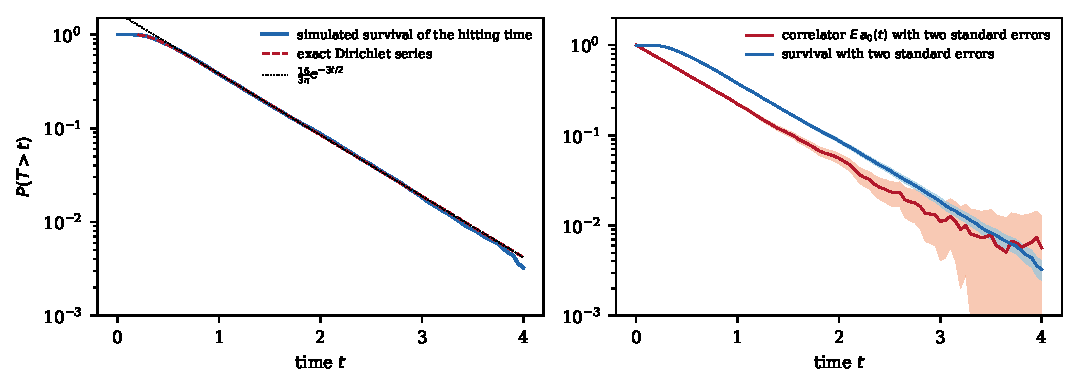
\includegraphics[width=0.85\textwidth]{figures/hitting_gap.pdf}
\caption[The gap of SU(2) from a hitting time]{Brownian motion on SU(2) started at the identity, twenty thousand paths. Left: the survival probability of the first hitting time of the equator, with the exact series of Proposition~\ref{prop:equator} and its leading term. Right: the survival probability and the correlator $\E a_0(t)=e^{-3t/2}$ from the same paths, each with a band of two standard errors. Both decay at the gap; the band of the survival probability stays narrow in relative terms for longer.}
\label{fig:hitgap}
\end{figure}

We simulated twenty thousand paths with step $0.002$, with a Brownian bridge correction for crossings between steps, without which the rate was biased down by about five percent in a single run. Both estimators use the same paths, and the errors of the effective mass are standard errors by the delta method with the empirical covariance of the two time points over those paths.

\begin{center}
\small
\begin{tabular}{lcc}
\toprule
estimator & window & estimate of the gap $\frac32$ \\ \midrule
hazard rate, exits over time at risk & $t>0.5$ & $1.452\pm0.012$ \\
hazard rate & $t>1$ & $1.497\pm0.017$ \\
hazard rate & $t>1.5$ & $1.491\pm0.025$ \\
effective mass of $\E a_0$ & $0$ to $0.5$ & $1.494\pm0.011$ \\
effective mass of $\E a_0$ & $0.5$ to $1$ & $1.520\pm0.027$ \\
effective mass of $\E a_0$ & $1$ to $1.5$ & $1.488\pm0.059$ \\
effective mass of $\E a_0$ & $1.5$ to $2$ & $1.27\pm0.11$ \\
effective mass of $\E a_0$ & $2$ to $2.5$ & $1.70\pm0.26$ \\
\bottomrule
\end{tabular}
\end{center}

At equal cost, for windows that start after $t=1$, the hitting time gives the gap three and a half times more precisely than the correlator, a factor of about twelve in sample size, and its error grows slowly as the window moves out where the correlator's grows exponentially (Figure~\ref{fig:hitgap}), because every surviving path contributes to the hazard estimate with a positive weight. The advantage does not extend to the correlator's earliest window: $0$ to $0.5$ is as good as the hazard rate ($\pm0.011$ against $\pm0.017$), because $a_0=\frac12\chi_2$ is an exact eigenfunction with no excited state, and the hazard rate is itself biased low when started earlier ($1.452\pm0.012$ from $t>0.5$). So the advantage needs a correlator whose early window is contaminated by excited states, as it is for a generic lattice observable, and we tested only this one, with twenty thousand paths and one seed.

\section{Is the hitting time approach useful for the mass gap?}

Useful in three ways, and limited in one.

\paragraph{\normalfont\scshape As an estimator.} A lattice simulation gives a sample of the Euclidean measure, and the Euclidean time direction of each configuration is, for infinite time extent, a stationary reversible Markov chain of time slices whose transition operator is the transfer matrix $\mathcal T$, normalised to have top eigenvalue $1$, positive by reflection positivity, with second eigenvalue $e^{-m}$. For a set $A$ of time slice configurations let $\lambda_A$ be the top of the spectrum of $\mathcal T$ compressed to functions vanishing on $A$, so that the probability of no visit to $A$ in $n$ consecutive slices decays like $\lambda_A^n$. The proof of Theorem~\ref{thm:hitgap}(i) applies to the form $\mu\big(f(1-\mathcal T)f\big)$ and gives
\[
1-e^{-m}\ \le\ \frac{1-\lambda_A}{\mu(A)} .
\]
The bound says something only when $(1-\lambda_A)/\mu(A)<1$. So run lengths in the time direction, for instance of the slice averaged plaquette staying below its median, give an upper bound on the mass gap from positive data. Upper bounds are the easy direction, as with every variational method, but this one needs no choice of operator basis and no fit window.

\paragraph{\normalfont\scshape In the Hamiltonian picture.} By Proposition~\ref{prop:groundstate} the gap is the spectral gap of the diffusion whose invariant law is the square of the ground state, so Theorem~\ref{thm:hitgap} restates positivity of the gap, uniformly in the volume, as a uniform bound on the rate at which that diffusion reaches sets of half the measure. This is a restatement and not a proof, but in terms of hitting times of large sets, for which coupling and drift methods exist, in the manner of Meyn and Tweedie~\cite{MT93}.

\paragraph{\normalfont\scshape With a reflection.} Proposition~\ref{prop:hitreflect} gives the gap of the odd sector as a Dirichlet eigenvalue when the fixed set of the reflection separates the state space. This holds for one group variable, as above, but not for a lattice field, whose fixed set has high codimension; it applies to reductions such as the plaquette law on a rung.

\paragraph{\normalfont\scshape The limitation.} The time of the hazard rate must be the physical time: the Monte Carlo time of a heat bath simulation has a gap of its own, which measures the algorithm. And the tangent approximation of Roberts and Shortland is a device for one dimensional diffusions; what carries over is the hazard rate as the object of study.

\section{Moderate deviations and exchangeability}\index{Rubin, H.}\index{Sethuraman, J.}

Between the central limit theorem, which describes deviations of a sum of $n$ terms at scale $\sqrt n$, and large deviations, at scale $n$, lies the range that Rubin and Sethuraman called moderate. For independent terms with variance $v$ and a finite moment generating function,
\[
\log P\big(\bar X_n-\E X_1>x_n\big)\sim-\frac{n x_n^2}{2v}\qquad\text{whenever}\quad n^{-1/2}\ll x_n\ll1,
\]
and with $x_n=\sqrt{c\,v\log n/n}$ the probability is $n^{-c/2}$ to leading order. Rubin and Sethuraman used this to define Bayes risk efficiency: the Bayes risk of a test is governed by errors of size $n^{-c}$, and so by moderate and not by large deviations. Three points of contact with this book.

\subsection*{The plaquette}

For the mean plaquette of two dimensional SU(2) everything is explicit: the cumulant function of one plaquette is $\log\big[I_1(\beta+s)/(\beta+s)\big]-\log\big[I_1(\beta)/\beta\big]$, and the rate function $I(x)$ is its Legendre transform. At $\beta=2.5$ the variance is $v=0.1341$ and the third cumulant is $\kappa_3=-0.0535$.

\begin{center}
\small
\begin{tabular}{ccccc}
\toprule
$n$ & deviation $x$ & $n\,I(x)$ & $I(x)\big/\frac{x^2}{2v}$ & with the Cram\'er term \\ \midrule
$10^3$ & $0.0134$ & 0.68 & 1.014 & 1.000 \\
$10^3$ & $0.0754$ & 23.0 & 1.085 & 1.010 \\
$10^5$ & $0.0065$ & 15.7 & 1.007 & 1.000 \\
$10^5$ & $0.0300$ & 346 & 1.031 & 1.002 \\
$10^7$ & $0.0119$ & 5382 & 1.012 & 1.000 \\
any & $0.3$ & $0.538\,n$ & 1.603 & 1.235 \\
\bottomrule
\end{tabular}
\end{center}

In the moderate range the Gaussian rate is right to a few percent and the first term of the Cram\'er series, $-\kappa_3x^3/(6v^3)$, removes the rest; at a fixed deviation neither is adequate. For an interacting lattice the corresponding statement is a hypothesis here and not a theorem: a moderate deviation principle for a dependent field needs mixing or cumulant bounds, a finite susceptibility alone does not give it for non Gaussian fields, and we cite no such result for lattice gauge theory. Under the hypothesis the Gaussian rate has $v$ replaced by the susceptibility, the sum of the plaquette covariances, which exponential clustering makes finite, and a failure of the Gaussian rate at moderate scale, such as a mean plaquette that fluctuates at order one, would signal a phase transition or a zero gap. The converse fails, since a finite susceptibility is weaker than a gap: moderate deviations are a necessary test under that hypothesis and not a sufficient one, and no theorem about the gap is claimed from them.

\subsection*{The one loop term of the ladder as a Cram\'er term}\index{Cram\'er series}

The second point is closer to the centre of the book. At small time the heat kernel on SU(2) with $u_2=e^{-3t/4}$ is
\[
K_t(\theta)\ \propto\ \frac{\theta}{\sin\theta}\,e^{-\theta^2/t}\,\big(1+O(e^{-c/t})\big),\qquad\log\frac{\theta}{\sin\theta}=\frac{\theta^2}{6}+\frac{\theta^4}{180}+\cdots .
\]
The Gaussian factor is the central limit theorem on the group. The factor $\theta/\sin\theta$ is the correction that matters when $\theta$ is large compared with $\sqrt t$ and small compared with one, the moderate range, and its first term changes the Gaussian rate from $1/t$ to $1/t-\frac16$.

\begin{remark}[One loop as curvature]\label{rem:cramerloop}
Match only the quadratic part of the exponent, dropping the quartic term and the images $O(e^{-c/t})$, and define the rate by this match. The $k$th power of $K_t$ has rate $k/t-k/6$ and the heat kernel $K_s$ has rate $1/s-\frac16$. They agree when $1/s=k/t-(k-1)/6$, that is
\[
s=\frac{t}{k}\Big[1-\Big(1-\frac1k\Big)\frac t6\Big]^{-1}=\frac tk\Big[1+\Big(1-\frac1k\Big)\frac t6+O(t^2)\Big],
\]
which is the first order term of Theorem~\ref{thm:expansion}. This is a leading order derivation and not a theorem.
\end{remark}

So the constant $\frac16$ that sets the one loop coefficient of the ladder, and through $(b^2-1)/(3b^2)$ the value $\frac14$ of $\beta-R(\beta)$ at $b=2$, is the first Cram\'er coefficient of Brownian motion on the group: the Ricci curvature of $S^3$ as we read it off the moderate deviations of the heat kernel. Asymptotic freedom on the ladder is a curvature correction to a Gaussian, visible only beyond the central limit scale. The next coefficient is not given by the quadratic match alone; the quartic term $\theta^4/180$ enters and Theorem~\ref{thm:expansion} is needed. The large deviation range, $\theta$ of order one, where the image sums and the antipode enter, is where total positivity failed in Chapter~\ref{ch:progress}.

\subsection*{Exchangeability and mixtures}\index{Zabell, S. L.}\index{exchangeability}
Exchangeability enters when the measure is a mixture. By de Finetti's theorem an exchangeable sequence is a mixture of independent ones, and Dinwoodie and Zabell \cite{DiZa92} showed that its large deviation rate is the lower envelope of the rates of the components over the support of the mixing measure,
\[
I(x)=\inf_{\xi\in\operatorname{supp}\pi}I_\xi(x).
\]
One consequence bears on the gap.

\paragraph{\normalfont\scshape Uniqueness of the vacuum.} If the infinite volume measure is a proper mixture of states with different plaquette expectations, the envelope vanishes at each of their plaquette expectations, the mean plaquette fluctuates at order one, and the Gaussian moderate deviation rate fails. The decomposition of a Gibbs measure into pure phases is de Finetti's theorem in another dress, and a unique vacuum, part of what a mass gap asserts, is the statement that the mixing measure is a point; so the moderate deviation test, under the hypothesis stated above, is a test for a nontrivial mixture.

\paragraph{\normalfont\scshape Assessment.} As tools of measurement, yes: for windows after $t=1$ the hazard rate estimator is more precise than the correlator in the one case we could test exactly, though not than the correlator's earliest window, and the moderate deviation scale gives sample sizes and, under the hypothesis above, a test for a unique phase. As structure, in one place: the one loop term of the ladder is a Cram\'er coefficient, which explains where $\frac16$ comes from. As a route to a proof, only as a restatement: Theorem~\ref{thm:hitgap} turns the gap into a uniform bound on hitting rates of large sets, a smaller and more probabilistic question than the one we started with, and one that is not answered here.

\section{Sufficient Statistics, Particle Learning and GBC}\label{ch:plgbc}\index{sufficient statistic}\index{particle learning}\index{generative Bayesian computation}

Three ideas from Bayesian computation have appeared in this book without being named together: sufficient statistics, which say what a lattice configuration knows about its coupling; particle learning, which carries sufficient statistics along a filter; and generative Bayesian computation, which learns the map from statistics to parameters from simulations. This section develops each for lattice gauge theory, runs them, and asks whether they are useful for the mass gap.

\subsection{Sufficient statistics of a lattice gauge field}

The Wilson measure is an exponential family in $\beta$ with the total action as its statistic:
\[
p_\beta(U)=\frac{e^{-\beta S(U)}}{Z(\beta)},\qquad S(U)=\sum_p\big(1-\tfrac12\operatorname{tr}U_p\big).
\]

\begin{proposition}\label{prop:suff}
\begin{enumerate}
\item[(i)] $S$ is a minimal sufficient statistic for $\beta$. The score is $\E_\beta S-S$, the Fisher information is $\operatorname{Var}_\beta(S)$, the specific heat times the volume up to a factor $\beta^2$ that depends on convention, and the maximum likelihood estimate solves $\E_{\hat\beta}S=S_{\mathrm{obs}}$.
\item[(ii)] For the family of single plaquette actions $\sum_p\sum_{n\ge2}c_n\chi_n(U_p)$ the character sums $T_n=\sum_p\chi_n(U_p)$ are sufficient, and maximum likelihood matches their expectations.
\item[(iii)] For a family of actions with one coupling for each loop shape in a finite list, the sums of those loops over the lattice are sufficient, and maximum likelihood matches their expectations.
\end{enumerate}
\end{proposition}

\begin{proof}
All three are the standard properties of exponential families: the density depends on the configuration only through the statistic, the log partition function is the cumulant generating function, and the likelihood equation equates the observed statistic with its mean.
\end{proof}

The proposition has a consequence that lattice practice uses without the name: matching is maximum likelihood. Parisi's effective coupling \cite{Pa80} of Chapter~\ref{ch:progress} matches the measured plaquette to its leading weak coupling formula, so it is the likelihood equation of the one parameter model whose mean plaquette is that formula, a moment estimator in a different model, and not the maximum likelihood estimate in the Wilson model, whose equation is $\E_{\hat\beta}S=S_{\mathrm{obs}}$. Swendsen's Monte Carlo renormalization group \cite{Sw79} is the method of moments for the family in (iii), and maximum likelihood for the blocked effective action when the list of loops is rich enough. The pseudolikelihood of Besag \cite{Be74,Be75} (Section~\ref{ch:slice}) replaces the global statistic by local conditional ones, the pairs $(k,a_0)$ of staple length and alignment at each link, and trades efficiency for the absence of a partition function.

\subsection{Two conjugate families and the ladder}

For class function laws on SU(2) there are two natural families, each closed under one of the two operations of the ladder. The Wilson, or von Mises Fisher, family $e^{\kappa\cos\theta}$ is closed under products ($f^k$ has concentration $k\kappa$) and is the conjugate family for bond moving, the Bayes update, with sufficient statistic $\cos\theta$. The heat kernel family $K_t$ is closed under convolution ($K_s*K_t=K_{s+t}$) and is the conjugate family for decimation, the predictive step, with sufficient statistic for prediction the time $t$. No one parameter family other than the trivial ones is closed under both: a law that is at once $e^{\kappa\cos\theta}$ and a heat kernel would have character coefficients $I_n(\kappa)/I_1(\kappa)$ and $e^{-(n^2-1)t/4}$ at once, which fails already at $n=3$ for every $\kappa>0$ (Section~\ref{ch:langlands} finds a larger family, indexed by the laws of an integer count, closed under the first operation and, conjecturally, the second).

That is the difficulty of the ladder in one sentence: in flat space the Gaussian family is closed under both operations and the coupling is marginal, and on the group the two families separate, the distance between them being the decrement. The heat kernel projection of Section~\ref{ch:verification} is what the filtering literature calls assumed density filtering. Proposition~\ref{prop:wilsonflow} concerns the heat flow of the Wilson law (monotone likelihood ratio in time exactly when $\kappa\le3/2$); it does not order the two families.

\subsection{How much does a statistic know?}\index{Fisher information}\index{Cram\'er Rao bound}

Sufficiency is a statement of no loss. It becomes useful when the loss of other summaries is measured, and the lattice offers a clean place to measure it. In two dimensions with free boundary conditions the plaquettes are independent with density proportional to $\sqrt{1-a^2}\,e^{\beta a}$ in $a=\frac12\operatorname{tr}U_p$, the mean is $u(\beta)=I_2(\beta)/I_1(\beta)$, and the Fisher information of one plaquette is
\[
i(\beta)=\operatorname{Var}_\beta(a)=1-\frac{3u(\beta)}{\beta}-u(\beta)^2 ,
\]
which falls from $\frac14$ at strong coupling to $3/(2\beta^2)$ at weak coupling. The Cram\'er Rao bound for $n$ plaquettes is $1/(n\,i(\beta))$.

We compared three estimators on six independent chains of three hundred configurations of a $16\times16$ torus at each of three couplings: maximum likelihood from the mean plaquette, Besag's pseudolikelihood of Section~\ref{ch:slice}, and the estimator that keeps one bit from each plaquette, whether $a>\frac12$.

\begin{center}
\footnotesize
\begin{tabular}{ccccc}
\toprule
$\beta$ & bound & max.\ likelihood & pseudolikelihood & one bit \\ \midrule
1 & 0.1327 & 0.1384\ \ (0.92$\pm$0.03) & 0.1397\ \ (0.91$\pm$0.04) & 0.1818\ \ (0.53$\pm$0.02) \\
2 & 0.1549 & 0.1589\ \ (0.95$\pm$0.02) & 0.1661\ \ (0.87$\pm$0.02) & 0.1989\ \ (0.61$\pm$0.02) \\
4 & 0.2306 & 0.2303\ \ (1.01$\pm$0.04) & 0.2513\ \ (0.85$\pm$0.03) & 0.2832\ \ (0.67$\pm$0.02) \\
\bottomrule
\end{tabular}
\end{center}

The first column of numbers is the Cram\'er Rao standard deviation; the others are means over the six replicates, with the efficiency (squared ratio to the bound) in brackets and its standard error over the replicates. Maximum likelihood is within three standard errors of the bound at $\beta=2$ and $4$, as expected for an exponential family in large samples, and $2.7$ standard errors below it at $\beta=1$, where the $256$ plaquettes of a torus are not independent. Pseudolikelihood is indistinguishable from maximum likelihood at $\beta=1$ and loses about eight percent at $\beta=2$ and sixteen percent at $\beta=4$ (two to three standard errors), because it discards the correlation between neighbouring links. A one bit summary loses a third to a half of the information (efficiency $0.53$ at $\beta=1$, $0.67$ at $\beta=4$), a warning for coarse summaries of blocked fields.

\paragraph{\normalfont\scshape Three uses of sufficiency.}\index{Rao Blackwell theorem}\index{Pitman Koopman Darmois theorem}\index{data processing inequality} Rao Blackwell: given the sum $V_\ell$ of its staples a link has the law $e^{\beta\operatorname{tr}(UV_\ell^\dagger)/2}$ with conditional mean $u(\beta|V_\ell|)\,V_\ell/|V_\ell|$, and conditioning on the staples is the multihit estimator of Parisi, Petronzio and Rapuano \cite{PPR}; the heat bath bound of Theorem~\ref{thm:heatbath} is its absolute value, so the gap in the sandwich of Section~\ref{ch:griffiths} is the price of the final triangle inequality, the phases of the staples. Pitman~\cite{Pi36}, Koopman~\cite{Ko36} and Darmois: a fixed dimensional sufficient statistic exists, among smooth families with fixed support, only for exponential families, and one step of the ladder takes the Wilson law out of $e^{\kappa\cos\theta}$, so every truncation, the heat kernel projection of Section~\ref{ch:verification} included, loses information in the sense of the table above; the projection keeps the fundamental character, the statistic the string tension reads, which is why it is the natural one. Data processing: blocking can only lose Fisher information about the fine theory; on a hierarchical lattice the block holonomies are sufficient for the long distance parameters, which is the exactness of Migdal and Kadanoff, while on $\mathbb Z^4$ they are not, and the comparison problem of Chapter~\ref{ch:sandwich} asks for two channels, one that keeps more and one that keeps less. Given its action, the Wilson measure is the Haar measure on a shell of constant action, and in large volume it concentrates on the shells near its mean action, the typical set of Cover and Thomas \cite{CT06}, through which nested sampling and the vertical likelihood of Section~\ref{ch:vertical} walk.

\subsection{Particle learning}

Particle learning, introduced by Carvalho, Johannes, Lopes and Polson \cite{CJLP}, is the filter for models with unknown static parameters that have conditional sufficient statistics. Each particle carries an essential state: the hidden state $x_m$, the sufficient statistics $s_m$ for the parameters given the path, and a draw of the parameters. One step resamples the particles with weights given by the predictive likelihood of the next observation, propagates the states from their conditional law given that observation, updates the statistics deterministically, and redraws the parameters from their conditional posterior. Section 20.6 of our Hilbert sixth book \cite{PS26h} proves that this step is exact at the level of laws, and discusses its degeneracy over long horizons.

The ladder is a model of this kind once we ask the statistical question that a lattice practitioner faces: given samples of blocked plaquettes at successive scales, what is the rate of running, and how uncertain is it? The state is the coupling $\beta_m$ at rung $m$, with $\beta_{m+1}=\beta_m-\delta+\sqrt q\,\varepsilon_m$. The observation is the mean $y_m$ of $n$ plaquette variables $\frac12\operatorname{tr}U_p$ at rung $m$, with mean $u_2(\beta_m)=e^{-3/(2\beta_m)}$ and variance $\big(\frac14(1+3e^{-4/\beta_m})-e^{-3/\beta_m}\big)/n$ in the heat kernel family. The parameters are the decrement $\delta$ and the innovation variance $q$, with a normal inverse gamma prior, and the sufficient statistics are the count, sum and sum of squares of the increments $\beta_m-\beta_{m+1}$ along the particle's path.

\begin{figure}[t]
\centering
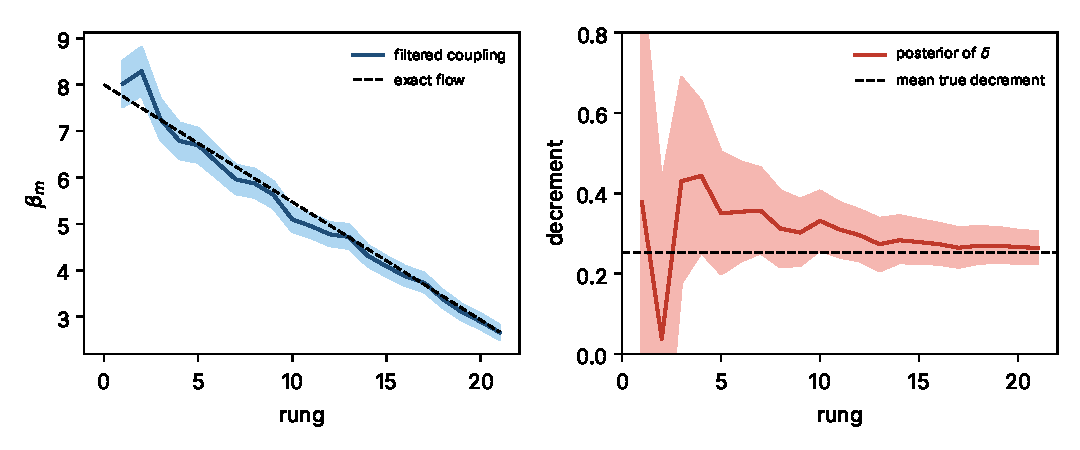
\includegraphics[width=0.85\textwidth]{figures/pl_ladder.pdf}
\caption[Particle learning of the decrement of the ladder]{Particle learning on the ladder with twenty thousand particles and four hundred plaquettes observed at each rung. Left: the filtered coupling with its ninety percent band, against the exact flow. Right: the posterior of the decrement $\delta$ as rungs accumulate, against the mean true decrement.}
\label{fig:plladder}
\end{figure}

We generated data from the exact, unprojected ladder started at $\beta=8$: twenty two rungs, four hundred plaquettes sampled at each. The true decrement varies slowly along the flow, from $0.2527$ to $0.2567$, with mean $0.2537$. Particle learning with twenty thousand particles, the predictive likelihood computed by the delta method, gives after twenty one steps a posterior median of $0.264$ for $\delta$ with ninety percent interval $[0.226,0.304]$ (Figure~\ref{fig:plladder}). Over five seeds the median is $0.261\pm0.004$ (standard error), with ninety percent endpoints $0.223\pm0.005$ and $0.300\pm0.004$; the run shown is seed $0$. Sixty one percent of the particles have distinct parents at the last resampling step; the number of distinct ancestors along the paths, which governs the accumulated sufficient statistics, was not measured, so we claim nothing about degeneracy.

The posterior of the decrement, the beta function at one loop accuracy, comes with an honest interval from data of the kind a simulation produces: twenty two rungs of four hundred plaquettes fix it to fifteen percent. The method does not need the ladder to be the true dynamics, and blocked ensembles from a real simulation would do.

\subsection{Generative Bayesian computation}

Generative Bayesian computation replaces the density of the posterior by a map. Simulate parameters from the prior and data from the model; reduce the data to a statistic; and train a generator, a function of the statistic and of a uniform variable, whose output has the conditional law of the parameter given the statistic. The posterior for observed data is then one forward pass. No likelihood and no partition function is evaluated, only simulations, which is exactly the situation of lattice gauge theory, where simulation is routine and $Z(\beta)$ is out of reach. By Proposition~\ref{prop:suff} nothing is lost if the statistic is sufficient.

We used it for the problem left open in Chapter~\ref{ch:sandwich}: the coupling fitted to a blocked field by pseudolikelihood depended on the blocking rule by a factor of more than three. Matching is the cure, and matching is what a generator trained on simulations does.

\paragraph{\normalfont\scshape Training and validation.} Four hundred and twenty simulations of a $4^4$ lattice, with the protocol of \texttt{gbc\_sim.py}, at couplings drawn uniformly from $[0.3,9]$, each reduced to the plaquette, the $1\times2$ loop and the $2\times2$ loop averaged over sixteen configurations. A gradient boosted quantile regression on the three loops and their logarithms is the generator for the median, trained on three hundred pairs; sixty pairs calibrate a ninety percent interval by split conformal prediction, and sixty test it. Over five replicate trainings and simulations the held out median absolute error in $\beta$ is $0.034\pm0.002$ and the interval covers the truth in $93\pm2$ percent of cases, against a nominal $90$; the coverage of one replicate has a standard error of four.

\paragraph{\normalfont\scshape Application.} Sixteen configurations of an $8^4$ lattice at each of five couplings were blocked to $4^4$ by five rules, plain decimation and decimation with the staples added with weights $0.1$, $0.2$, $0.3$ and $0.5$, and the same three statistics were passed to the generator. The blocked $8^4$ and trained $4^4$ lattices have the same number of sites, so finite size effects are matched, which is Swendsen's two lattice design \cite{Sw79}. As a check that the blocked ensemble is close to a Wilson ensemble we also matched each loop separately; the spread of the three matched couplings measures the distance from the Wilson family.

\begin{center}
\small
\begin{tabular}{cccccc}
\toprule
$\beta$ & smearing & generator, $\beta'$ & 90\% interval & spread of loops & $\beta-\beta'$ \\ \midrule
2.2 & 0.2 & $1.39\pm0.03$ & $[1.34,1.44]$ & $0.12\pm0.01$ & $0.81\pm0.03$ \\
2.5 & 0 & $1.21\pm0.01$ & $[1.17,1.24]$ & $0.51\pm0.01$ & $1.30\pm0.01$ \\
2.5 & 0.2 & $2.13\pm0.02$ & $[2.01,2.25]$ & $0.04\pm0.004$ & $0.38\pm0.02$ \\
2.5 & 0.5 & $2.33\pm0.02$ & $[2.19,2.47]$ & $0.19\pm0.01$ & $0.17\pm0.02$ \\
3 & 0.2 & $2.62\pm0.01$ & $[2.44,2.80]$ & $0.07\pm0.003$ & $0.38\pm0.01$ \\
\bottomrule
\end{tabular}
\end{center}

\begin{figure}[t]
\centering
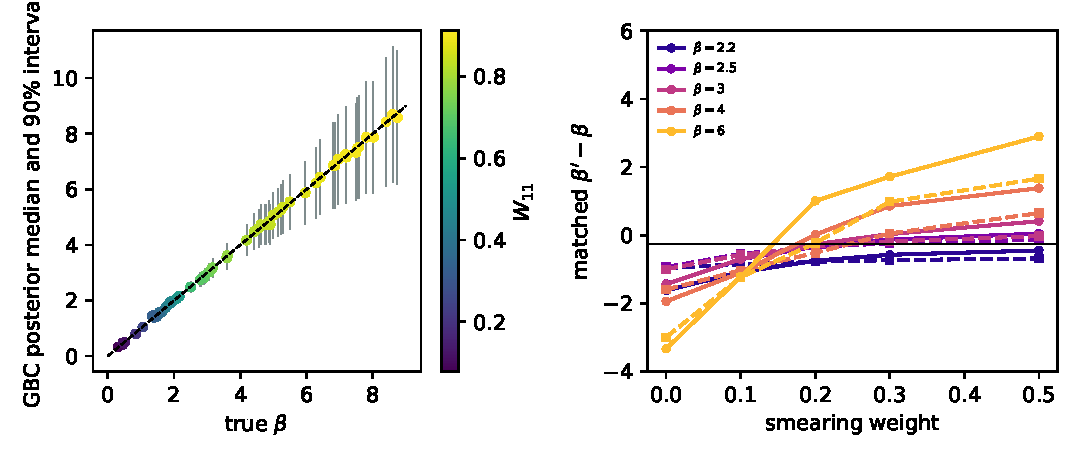
\includegraphics[width=0.85\textwidth]{figures/gbc_match.pdf}
\caption[GBC matching for a blocked lattice]{Left: the generator's posterior median and calibrated ninety percent interval against the true coupling on sixty held out $4^4$ simulations, coloured by the plaquette. Right: the shift $\beta'-\beta$ of the matched coupling of blocked $8^4$ ensembles as a function of the smearing weight of the blocking rule, matched by the plaquette (circles, solid) and by the $2\times2$ loop (squares, dashed); the horizontal line is $-0.26$.}
\label{fig:gbcmatch}
\end{figure}

Three things come out (Figure~\ref{fig:gbcmatch}); each row of the table is the mean over five replicate trainings and simulations, each with a blocked ensemble of sixteen configurations, and the interval column is the mean of the five ninety percent posterior intervals of the generator, which is its posterior uncertainty and not a replicate error. First, the dependence on the blocking rule shrinks: at $\beta=2.5$ pseudolikelihood gave fitted couplings from $0.87$ to $2.81$ across rules, matching gives $1.21$ to $2.33$, and the internal check selects among them, the three loops agreeing to $0.04$ at smearing weight $0.2$ and disagreeing by $0.12$ to $0.51$ at the others, so that the selected ensemble is, to the resolution of three loops, a Wilson ensemble at $\beta'=2.13\pm0.02$ (mean and standard error over the five replicates). Second, the shift at the selected rule is of the right size: $0.38\pm0.02$ at $\beta=2.5$ and $0.38\pm0.01$ at $\beta=3$ (over five replicates), against $0.21$ from the string tension data, $0.27$ from two loop perturbation theory and $0.26$ from the ladder; one step on a $4^4$ lattice with three loops overestimates it by about a half, which Monte Carlo renormalization studies remove with several steps on larger lattices. Third, the method fails gracefully: for $\beta\ge4$ the $4^4$ lattice is deep in its finite volume regime and no rule makes the three loops agree to better than about $0.1$ on average over replicates, which the spread reports.

\subsection{GBC against an exact posterior}

A generator is only as good as its statistic, and the two dimensional lattice lets us say so with numbers, because the posterior there is known in closed form. With $n=256$ independent plaquettes and a uniform prior on $[0.5,6]$, the posterior density of $\beta$ is proportional to $\big(\beta/I_1(\beta)\big)^n e^{n\beta\bar a}$ and depends on the data through the mean $\bar a$ alone. We trained quantile generators on six thousand simulated data sets, once with the sufficient statistic as input and once with the one bit summary, and compared five quantiles with the exact ones on six hundred fresh data sets, from one training run (seed $3$ of \texttt{gbc\_exact.py}), so the quantile errors and widths below carry no replicate error.

\begin{center}
\small
\begin{tabular}{lccc}
\toprule
input & quantile error & 90\% width & coverage \\ \midrule
sufficient statistic & 0.024 to 0.038 & 0.644 & 0.87 \\
one bit summary & 0.119 to 0.135 & 0.808 & 0.91 \\
exact posterior & 0 & 0.653 & 0.905 \\
\bottomrule
\end{tabular}
\end{center}

\begin{figure}[t]
\centering
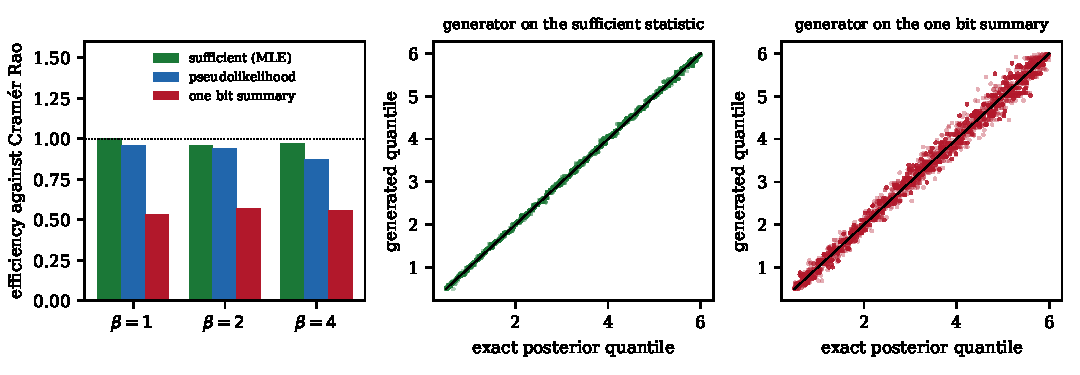
\includegraphics[width=0.85\textwidth]{figures/suff_gbc.pdf}
\caption[Sufficiency, efficiency and GBC]{Left: efficiency of three estimators of the coupling of two dimensional SU(2) against the Cram\'er Rao bound. Centre and right: the fifth, fiftieth and ninety fifth percentiles produced by a quantile generator against the exact posterior percentiles, when the generator is fed the sufficient statistic and when it is fed a one bit summary of each plaquette.}
\label{fig:suffgbc}
\end{figure}

With six hundred test sets a coverage has a standard error of about $0.012$: the exact interval covers $0.905\pm0.012$, the sufficient statistic generator at $0.87$ undercovers by two to three standard errors, and the one bit generator at $0.91$ is not distinguishable from $0.90$. With the sufficient statistic the generator reproduces the exact posterior to about a twentieth of its width; the residual is the training error of a boosted tree and presumably falls with more simulations, which we did not test. With the lossy statistic it is still calibrated and its intervals are a quarter wider. Both facts are general: a generator trained on a statistic $T$ targets the posterior given $T$, which has the right coverage, and what is lost is width, in the proportion that the Fisher information of $T$ falls short. The ratio of widths, $0.808/0.653=1.24$, lies within the range $1/\sqrt{0.67}=1.22$ to $1/\sqrt{0.53}=1.37$ that the efficiency table predicts, the prior truncating both posteriors. The practical rule is that of Proposition~\ref{prop:suff}: feed the generator the loop sums of the action family one is matching to, and nothing coarser (Figure~\ref{fig:suffgbc}).

\subsection{A generator for the gap}

The second role listed at the end of this section, the gap as a parameter, can be tried at once on synthetic correlators. Take $C(\tau)=A_1e^{-m\tau}+A_2e^{-M\tau}$ plus noise at $\tau=1,\dots,10$, with a prior over the gap $m\in[0.2,1.2]$, the amplitudes, the excited level $M-m\in[0.5,2]$ and the noise level between $10^{-3}$ and $10^{-2}$. Six thousand simulated correlators train a quantile generator for $m$; two thousand calibrate its interval; two thousand test it against the effective mass $\log C(\tau)/C(\tau+1)$.

\begin{figure}[t]
\centering
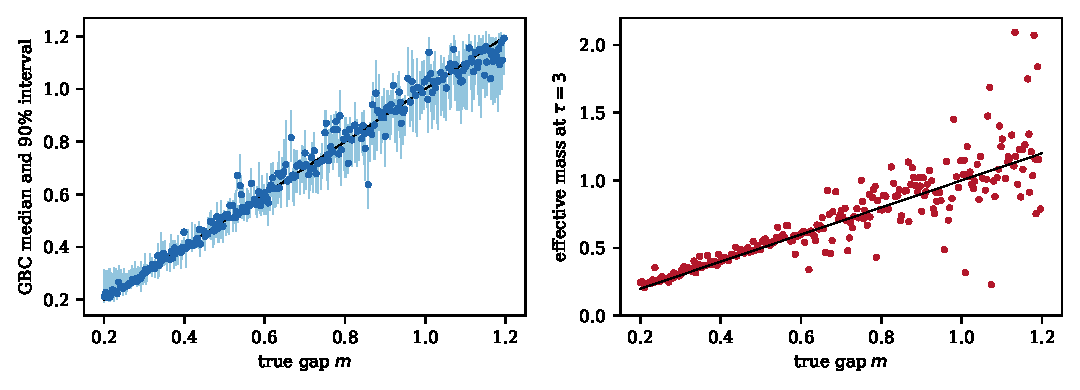
\includegraphics[width=0.85\textwidth]{figures/gbc_gap.pdf}
\caption[A generator for the gap]{Left: the posterior median and calibrated ninety percent interval for the gap produced by a generator trained on simulated two level correlators, against the truth. Right: the effective mass at $\tau=3$ for the same correlators.}
\label{fig:gbcgap}
\end{figure}

The generator's median error is $0.018$, against $0.045$ for the effective mass at $\tau=3$ and $0.091$ at $\tau=5$ (over the $90$ percent of cases in which it is defined); its calibrated ninety percent interval has mean width $0.15$ and covers the truth in $92$ percent of test cases (Figure~\ref{fig:gbcgap}). These are errors over two thousand test correlators from one training run. Over five training runs the median error is $0.0193\pm0.0004$ against $0.0455\pm0.0004$ and $0.097\pm0.003$ for the effective mass at $\tau=3$ and $5$, the interval covers $0.905\pm0.004$ with mean width $0.151\pm0.002$ (standard errors over seeds). The generator uses all ten times with weights learned from the prior, and that is also its limitation: the answer is a posterior under a prior on spectra with two levels, and under a prior that allows a continuum starting at zero no finite set of correlator values bounds the gap below. A generator moves the assumption into the open; it does not remove it.

\subsection{Transformers inside GBC}\index{transformer}\index{attention}

Can a transformer be the generator? A lattice ensemble is a set, and the natural network embeds each element as a token, lets the tokens attend to one another, and pools. By Proposition~\ref{prop:suff} the tokens should be the characters $\chi_n$ of the loops, which makes the network gauge invariant, and by the Pitman Koopman Darmois theorem attention, which can form products of tokens, may be needed once the action leaves the exponential family; with heat kernel weights it may act as a decimation step, and a transformer over plaquette tokens as a learned ladder. With no deep learning library available we tested the two ingredients in their simplest forms, on the two dimensional problem where the posterior is exact.

\paragraph{\normalfont\scshape Pooling.} Each of the $256$ plaquettes is embedded by its characters $\chi_2/2,\dots,\chi_9/9$ and the tokens are averaged, which is attention with uniform weights. A boosted quantile head is trained on the eight pooled coordinates. Only the first is sufficient; the head must find that out.

\paragraph{\normalfont\scshape In context attention.} A single attention head with the test ensemble as query and five thousand simulated ensembles as context: the weight on a context ensemble is $\exp(-\frac12|W(s-s_i)|^2)$ with $s$ the pooled vectors and $W$ diagonal with two free scales, one for the first coordinate and one shared by the other seven, chosen from a grid of twelve pairs on a validation split. The posterior quantiles are the attention weighted quantiles of the context couplings. This is the prior fitted network idea~\cite{MHAGH22} in one layer, and it is a kernel smoother.

The table gives means over five seeds, each with five thousand training and five hundred test sets, the same sets in every row; the standard error of each mean quantile error is about $0.001$, of each width $0.002$ to $0.004$ and of each coverage $0.003$ to $0.006$.

\begin{center}
\small
\begin{tabular}{lccc}
\toprule
generator & quantile error & 90\% width & coverage \\ \midrule
boosted head on the sufficient statistic & 0.026 to 0.038 & 0.648 & 0.88 \\
boosted head on eight pooled characters & 0.032 to 0.050 & 0.656 & 0.88 \\
attention head on eight pooled characters & 0.016 to 0.026 & 0.668 & 0.89 \\
exact posterior & 0 & 0.648 & 0.90 \\
\bottomrule
\end{tabular}
\end{center}

The attention head is the most accurate of the three, but what it chose was partly built in: the grid gave the first coordinate its own scale and the other seven a shared one, so the split between signal and noise was fixed by hand and not learned. Within the grid the validation step chose $0.03$ standard deviations for the first coordinate, the lower end of the grid, and infinity for the shared scale, in all five seeds; to claim that attention finds the sufficient statistic one would have to search eight free scales, which we did not do. The boosted head given the same eight inputs was about thirty percent worse than on the sufficient statistic alone, on the same data sets ($0.040$ against $0.031$); we did not test the natural reason, that it spends splits on the noise coordinates.

So the answer is yes in design and in a toy, with cautions: the toy is an exponential family, where the answer was known, and the case for attention is the blocked ensemble, where no finite statistic is sufficient and a trained network is needed, for which the flows of Kanwar and coauthors \cite{Kan20} and the convolutional networks of Favoni and coauthors \cite{Fav22} are the starting point. A transformer generator inherits every limitation of GBC: it computes posteriors under a simulated prior and proves nothing.

\subsection{Are GBC methods useful?}

Yes, for computation and for diagnosis, in three roles. Amortised matching: a generator trained once on small lattice simulations turns any blocked ensemble into a posterior for its effective coupling in a forward pass (twenty five posteriors in under a second, from about four minutes of parallel simulation), and extended to the character coefficients of a plaquette law it is the empirical ladder that Chapter~\ref{ch:sandwich} asked for. The gap as a parameter: a generator trained on simulated correlators with known spectra would give the posterior of the estimator of Chapter~\ref{ch:estimation} instantly and make the dependence on the prior over spectra explicit. Learning the block spin map: a generator trained on pairs of fine and blocked summaries is a learned ladder, which would show where in the bracket the truth lies for any blocking rule.

For a proof they are not useful directly: a trained generator is not a theorem, and its guarantees, such as the Bernstein von Mises transfer of our Hilbert sixth book \cite{PS26h}, concern statistical accuracy and not rigour of bounds. Their indirect use is real, though. The comparison problem needs a blocking rule and a pair of brackets, and there are infinitely many candidates. A learned ladder is a fast way to search that space for a rule under which the blocked law stays in a low dimensional family and the sandwich holds with room to spare, before any attempt is made to prove it. The pooled character model of the transformer experiment is of the kind suggested by quantum Bayesian computation \cite{PSX23}; Section~\ref{ch:quantum} takes the question up.

\section{Quantum Bayesian Computation and the Gap}\label{ch:quantum}\index{quantum Bayesian computation}\index{von Neumann measurement}\index{quantum Fourier transform}\index{Kogut Susskind Hamiltonian}

The mass gap is an eigenvalue difference. Monte Carlo infers it from a decay; a quantum computer would measure it. This section asks what our work on quantum Bayesian computation gives the problem, and what it gives the classical computations of this chapter as an architecture.

\subsection{Von Neumann's principle}

Our paper with Jianeng Xu \cite{PSX23} organises Bayesian computation round von Neumann's principle of measurement: a quantity of interest is written as $\operatorname{tr}(\rho\,Q)$ for a density operator $\rho$ and an observable $Q$, and is obtained by evolving a physical system and measuring it. Data enter through a feature map $x\mapsto\rho(x)$ into density matrices, a model is $f_W(x)=\operatorname{tr}(\rho(x)W)$, the kernel is $k(x,x')=\operatorname{tr}(\rho(x)\rho(x'))$, and since the model is linear in $W$, fitting $W$ is a convex problem, whose solution by the representer theorem lies in the span of the $\rho(x_i)$.

In most of statistics the trace formula is an analogy. In lattice gauge theory it is the definition. By reflection positivity a correlation on a lattice of temporal extent $N_t$ is
\[
\langle O_1(0)O_2(k)\rangle=\frac{\operatorname{tr}\big(\mathcal T^{N_t-k}O_1\,\mathcal T^kO_2\big)}{\operatorname{tr}\mathcal T^{N_t}},\qquad \mathcal T=e^{-H},
\]
with $\mathcal T$ the transfer operator, and the mass gap is the difference of the two lowest eigenvalues of $H$. The estimation problem of the earlier chapters, the gap from the decay of a correlator, is the classical shadow of a measurement of that difference. So of all the problems to which the methods of \cite{PSX23} apply, this is one where the quantum formulation is native and not a translation.

\subsection{One plaquette as a quantum system}\label{sec:oneplaquette}

The smallest example can be solved, and it shows the two regimes of the full problem. In the Hamiltonian formulation of Kogut and Susskind \cite{KS75} a single plaquette of SU(2), restricted to gauge invariant states, which are class functions, has
\[
H_\lambda=-\lambda\,\Delta+\frac1\lambda\,(1-\cos\theta),
\]
with $\Delta$ the Laplacian of this book, whose eigenvalue on the character $\chi_n$ is $-\frac14(n^2-1)$, and $\lambda$ proportional to the square of the coupling, with a constant fixed by the normalisation of the Hamiltonian.

\begin{proposition}[one plaquette]\label{prop:oneplaquette}
In the orthonormal basis $\chi_1,\chi_2,\dots$ of class functions the operator $H_\lambda$ is the tridiagonal matrix with diagonal entries $\frac14\lambda(n^2-1)+1/\lambda$ and off diagonal entries $-1/2\lambda$. Its gap is $\frac34\lambda+O(1/\lambda^3)$ as $\lambda\to\infty$ and tends to $\sqrt2$ as $\lambda\to0$.
\end{proposition}

\begin{proof}
The Casimir is diagonal, and $\cos\theta\,\chi_n=\frac12(\chi_{n+1}+\chi_{n-1})$ with $\chi_0=0$, since $\chi_2\chi_n=\chi_{n+1}+\chi_{n-1}$. For large $\lambda$ the potential is a bounded perturbation of the Casimir, whose lowest levels are $0$ and $\frac34\lambda$; the first order shifts of the two levels are equal, both $1/\lambda$ since $\cos\theta$ has no diagonal entries, and the second order shifts are of order $\lambda^{-2}$ over a level spacing of order $\lambda$. For small $\lambda$ the ground state concentrates at the identity, where $1-\cos\theta=\frac12\theta^2$ and $-\Delta$ is a quarter of the Laplacian of $\mathbb R^3$ in the length $\theta$; the operator $\frac14\lambda\,p^2+q^2/2\lambda$ is a harmonic oscillator of frequency $1/\sqrt2$, and the first excited radial state lies two quanta above the ground state.
\end{proof}

So the gap of one plaquette is never small: it is $\frac34\lambda$ at strong coupling, where it is the first Casimir, the number that appears all through this book, and $\sqrt2$ at weak coupling, with a minimum near $1.1$ between. Table~\ref{tab:oneplaquette} and Figure~\ref{fig:quantumplaquette} give the numbers. A single plaquette has no infrared problem; the problem of four dimensions is that infinitely many of them share links.

\begin{table}[t]
\centering\small
\begin{tabular}{rcccc}
\toprule
$\lambda$ & gap & $\frac34\lambda$ & characters kept & count of ground state \\ \midrule
$8$ & $6.0009$ & $6.0000$ & $3$ & $0.04$ \\
$2$ & $1.5569$ & $1.5000$ & $5$ & $0.75$ \\
$1$ & $1.0982$ & $0.7500$ & $6$ & $3.09$ \\
$0.5$ & $1.2394$ & $0.3750$ & $9$ & $8.78$ \\
$0.1$ & $1.3824$ & $0.0750$ & $20$ & $54.06$ \\
$0.02$ & $1.4079$ & $0.0150$ & $46$ & $280.34$ \\
\bottomrule
\end{tabular}
\caption[One plaquette in the Hamiltonian formulation]{The gap of $H_\lambda$, the number of characters that must be kept for the gap to be right to $10^{-8}$, and the count $E[1/(1-\cos\theta)]-2$ of the ground state density. The weak coupling limit of the gap is $\sqrt2=1.4142$.}
\label{tab:oneplaquette}
\end{table}

\begin{figure}[t]
\centering
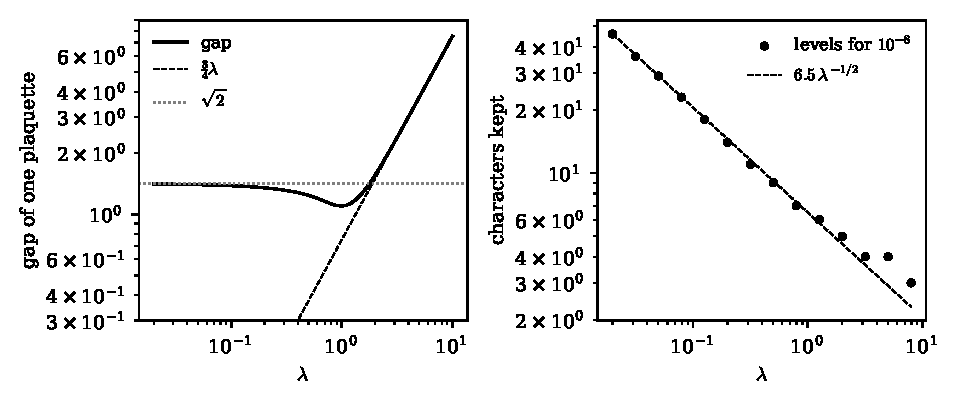
\includegraphics[width=0.85\textwidth]{figures/quantum_plaquette.pdf}
\caption[The gap and the truncation of one plaquette]{Left: the gap of one plaquette against $\lambda$, with its strong coupling asymptote $\frac34\lambda$ and its weak coupling limit $\sqrt2$. Right: the number of characters needed for an error of $10^{-8}$ in the gap, against $6.5\,\lambda^{-1/2}$.}
\label{fig:quantumplaquette}
\end{figure}

\paragraph{\normalfont\scshape Truncation and the count.} A quantum simulation keeps finitely many levels on each link, and the table says how many: at weak coupling the number of characters needed grows like $6.5\,\lambda^{-1/2}$ for eight figures. The count of Proposition~\ref{prop:observable} on the square of the ground state (in its class by Corollary~\ref{cor:vacuumcount}) agrees with $4\sqrt2/\lambda-\frac52$ to $0.003$ for $\lambda\le0.05$ (a numerical fit; the leading term is the harmonic oscillator value), so the levels a link needs grow like the square root of its count, about $2.7\sqrt M$. The latent count of Chapter~\ref{ch:counts}, introduced as a mixing variable and found to be an observable, is here also the measure of the register a link requires.

\subsection{The vacuum of one plaquette has real zeros}\label{sec:vacuumzeros}

The transfer operator of the plaquette over a short time $\epsilon$ is, by Trotter's formula, a heat flow between two multiplications,
\[
T_\epsilon=e^{-\epsilon V/2}\,e^{\epsilon\lambda\Delta}\,e^{-\epsilon V/2},\qquad V=\frac1\lambda(1-\cos\theta),
\]
and each factor is one of the operations of Chapter~\ref{ch:zeros}. That has a consequence for the vacuum.

\begin{proposition}[the vacuum has real zeros]\label{prop:vacuumzeros}
The ground state $\psi_0$ of $H_\lambda$, as an entire function of $x=\cos\theta$, has only real zeros, all in $(-\infty,-1]$. Hence
\[
\psi_0(x)=\psi_0(0)\,e^{ax}\prod_m\Big(1+\frac{x}{\gamma_m}\Big),\qquad a\ge0,\ \gamma_m\ge1,
\]
and $\psi_0(0)/\psi_0(x)$ is the Laplace transform in $x$ of a generalized gamma convolution with drift $a$ and unit Thorin atoms at the $\gamma_m$. The same holds for the vacuum density $\psi_0^2$, with atoms of weight two.
\end{proposition}

The proof needs one estimate, uniform in the Trotter step. In the character basis write $X$ for multiplication by $\cos\theta$, the tridiagonal matrix with entries $\frac12$, put $\kappa=\epsilon/2\lambda$, and write
\[
T_\epsilon=M\,D\,M,\qquad M=e^{\kappa(X-1)},\qquad D=\operatorname{diag}\big(e^{-\epsilon\lambda(n^2-1)/4}\big).
\]

\begin{lemma}[domination]\label{lem:domination}
For $m\epsilon=s$ every entry of $T_\epsilon^m$ satisfies
\[
0\le\big(T_\epsilon^m\big)_{nj}\le b_n(s)=e^{-s\lambda(n^2-4)/16}+e^{s/\lambda}\,\frac{(s/\lambda)^{\lceil n/2\rceil}}{\lceil n/2\rceil!},
\]
and every row sum is at most $1$. If $c\ge0$ is a unit vector with $T_\epsilon c=\mu c$, then $c_n\le\mu^{-m}\,b_n(s)^{1/2}$.
\end{lemma}

\begin{proof}
All of $X$, $M$ and $D$ have nonnegative entries, and $X$ has row sums at most $1$, so the same is true of $M$ and of $T_\epsilon$. Expand each factor $M$ in powers of $X$: the entry $(n,j)$ of $T_\epsilon^m$ becomes a sum over nearest neighbour paths from $j$ to $n$, each step with weight $\frac12$, interleaved with the diagonal factors. Paths that stay at or above level $n/2$ collect from each of the $m$ factors $D$ at most $e^{-\epsilon\lambda(n^2/4-1)/4}$, and the rest of their weight is an entry of $e^{2m\kappa(X-1)}$, which is at most $1$. Paths that go below $n/2$ have at least $\lceil n/2\rceil$ steps; dropping the factors $D$, which are at most $1$, the total weight of paths with $r$ steps is at most $(2m\kappa)^r/r!$, and $2m\kappa=s/\lambda$. Summing over $r\ge\lceil n/2\rceil$ gives the second term. For the eigenvector, $c=\mu^{-m}T_\epsilon^mc$ and, by the Cauchy and Schwarz inequality, $\sum_j(T_\epsilon^m)_{nj}c_j\le\big(\sum_j(T_\epsilon^m)_{nj}^2\big)^{1/2}\le\big(\max_j(T_\epsilon^m)_{nj}\big)^{1/2}$, the row sum being at most $1$.
\end{proof}

\begin{proof}[Proof of Proposition~\ref{prop:vacuumzeros}]
The constant function is in $\mathcal L$. Multiplication by $e^{\kappa x}$ is a limit of multiplications by $(1+x/\gamma)^m$ with $\gamma=m/\kappa\ge1$, and $\mathcal L$ is closed under products; the heat flow preserves $\mathcal L$ by Theorem~\ref{thm:zeros}. So every $T_\epsilon^k1$ is a locally uniform limit, in the complex variable $x$, of members of $\mathcal L$.

A function $\sum_nc_n\chi_n$ with $c_n\ge0$ is bounded on the ellipse through $\cosh\tau$ with foci $\pm1$ by its value $\sum_nc_n\sinh(n\tau)/\sinh\tau$ at $\cosh\tau$, since $\chi_n(\cos\theta)=\sum_ke^{i(n-1-2k)\theta}$. By Lemma~\ref{lem:domination} with $s=1$ the coefficients of the normalised iterates $T_\epsilon^k1/\|T_\epsilon^k1\|$, for $k\ge1/\epsilon$, and of the ground state $\phi_\epsilon$ of $T_\epsilon$, are bounded by a constant times $b_n(1)^{1/2}$, uniformly in $k$ and in $\epsilon\le1$: the factor $\mu^{-m}$ is $e^{E_\epsilon}$ with $E_\epsilon$ bounded, and for the iterates the ratio $\|T_\epsilon^{k-m}1\|/\|T_\epsilon^k1\|$ is bounded because the iterates keep an overlap with $\phi_\epsilon$ that is bounded below. Since $b_n(1)^{1/2}$ decays faster than any exponential, these families are uniformly bounded on every compact set of the $x$ plane, hence normal. The iterates converge in $\ell^2$ to $\phi_\epsilon$, because $T_\epsilon$ is compact, positivity improving and has a simple top eigenvalue; and $\phi_\epsilon\to\psi_0$ in $\ell^2$ as $\epsilon\to0$ by Trotter's formula and the simplicity of the ground state of $H_\lambda$. A normal family with convergent coefficients converges locally uniformly, and Hurwitz's theorem gives $\psi_0$ only real zeros, all in $(-\infty,-1]$. An entire function that is such a limit of polynomials with zeros on a half line has the displayed form, by the theorem of Laguerre and P\'olya; and the reciprocal of $e^{ax}\prod(1+x/\gamma_m)$ is the Laplace transform of a drift plus a sum of independent exponential variables.
\end{proof}

As a check on the conclusion, independent of the proof: with the ground state computed to $160$ digits (\texttt{vacuum\_zeros.py}) in a basis of $70$ to $110$ characters, the number of zeros in a disc, counted by the argument principle, equals the number of sign changes on the real axis below $-1$: one zero in $|x|<12$ at $\lambda=2$, at $x=-6.731$; five in $|x|<6$ at $\lambda=\frac12$, the nearest at $-1.206$; fifteen in $|x|<2.5$ at $\lambda=\frac1{10}$, the nearest at $-1.0065$. At $60$ digits the last count comes out wrong, a warning of the kind recorded in Chapter~\ref{ch:zeros}.

\begin{corollary}\label{cor:vacuumcount}
The vacuum density $\psi_0^2$ of one plaquette is a mixture $\sum_j\pi(j)f_j$ with a log concave count law $\pi$, whose mean is the count of Table~\ref{tab:oneplaquette}.
\end{corollary}

\begin{proof}
$\psi_0^2$ is in the closure of $\mathcal L$, and Proposition~\ref{prop:Llogconcave} and Proposition~\ref{prop:observable} pass to limits.
\end{proof}

So the vacuum of the smallest gauge system belongs to the class in which the heat kernel lives, with zeros that crowd toward the antipode as the coupling weakens, and its reciprocal has the Thorin form on which this book began. The proof used nothing about the potential except that $e^{-\epsilon V}$ is, up to a constant, a Wilson weight; whether the same holds for other single plaquette actions whose Boltzmann factor is in the closure of $\mathcal L$, the heat kernel action among them, is not shown here. For several plaquettes the statement to aim at is the same one, in each plaquette variable separately, and that is a question about how sharing a link interacts with real zeros: Conjecture~\ref{conj:Lclosed} is the case of two.

\subsection{The ladder alternates between two bases}

The two halves of a rung are diagonal in different bases: decimation is a convolution, diagonal in characters ($u_n\mapsto u_n^{\,p}$), and bond moving a pointwise product, diagonal in the group variable, with the matrix $u_n(j+1)$ of Chapter~\ref{ch:counts} as the change of basis between counts and characters. That is the pattern of the quantum Fourier transform models of \cite{PSX23}: layers each trivial in their own basis, joined by a fixed transform. Nothing in the ladder needs a quantum computer, since it is a commutative computation; the noncommutative one is the lattice $\mathbb Z^4$, where a plaquette shares each of its links with five others, and the comparison problem of Chapter~\ref{ch:sandwich} asks how far the true blocking map is from one that is diagonal in alternate bases.

\subsection{Band limited models as an architecture for GBC}

A model $\operatorname{tr}(\rho(x)W)$ with a fixed encoding is a finite Fourier series in the data. For a gauge invariant model of a lattice gauge field the Peter and Weyl theorem says it is a combination of characters $\chi_n$ of plaquettes and longer loops up to a band $N$, and the coherent state kernel, Gaussian in \cite{PSX23}, is on the group the heat kernel $K_t(UV^{-1})$, positive definite because its character coefficients are positive. So the quantum architecture, run on a classical machine, is: Peter and Weyl features to a band $N$, pooled over the lattice; products of a few copies of the pooled vector, which is what several copies of the state give; and a linear readout fitted by ridge regression, a convex problem.

We tried it on the test problem of Section~\ref{ch:plgbc}: $256$ independent Wilson plaquettes, a uniform prior on $\beta$, and the exact posterior median as the target. The readout is a quadratic polynomial in the pooled characters plus the cube of the first, fitted on $4000$ simulated sets and tested on $500$.

\begin{center}
\small
\begin{tabular}{lcccc}
\toprule
band $N$ & $1$ & $2$ & $4$ & $8$ \\ \midrule
features & $4$ & $7$ & $16$ & $46$ \\
error against the exact median & $0.040$ & $0.033$ & $0.031$ & $0.035$ \\
\bottomrule
\end{tabular}
\end{center}

The error is the mean absolute one, from one seed, so differences in the third decimal are not resolved. The first character is sufficient for this model, so in principle band $1$ is enough, and the small gain from bands $2$ and $4$ is the polynomial readout borrowing nonlinearity from the higher characters; at band $8$ the extra features begin to cost. The attention head of Section~\ref{ch:plgbc}, at $0.016$ at the median, does better than any of these; the boosted head on the same pooled characters, at $0.032$, does not. The comparison is between different training sets ($4000$ against $5000$) with the same $n$ and prior. So against the attention head the convex readout is the limiting factor here and not the features. The advice that survives is about the feature layer: put the invariance and the band limit into the encoding, where the theory says what they are, and spend the flexibility on the readout. The paper notes that convex training avoids the flat landscapes met by deep parameterised circuits; the experiment says that on this problem one pays for the convexity with up to a factor of two in error.

\subsection{What a quantum computer could and could not do}

\paragraph{\normalfont\scshape Could.} Evolve a truncated Kogut and Susskind Hamiltonian and read the gap as a phase. Phase estimation \cite{Ki95}, a standard result of quantum computation, to precision $\varepsilon$ needs evolution for a time of order $1/\varepsilon$, so a gap $m$ is resolved in time of order $1/m$, against the classical need for correlators at separations of several $1/m$ with noise that does not fall with the signal. Real time evolution and matter at finite density, where Monte Carlo has a sign problem, are the cases usually argued for.

\paragraph{\normalfont\scshape Could not.} Prove a gap. The ground state must be prepared, and adiabatic preparation \cite{FGGS00}, by the adiabatic theorem, takes a time that grows as an inverse power of the gap along the path, so the cost of the measurement depends on the quantity measured; at weak coupling the gap in lattice units is expected, from asymptotic freedom, to be exponentially small in $\beta$ and the lattice must be exponentially large. And a measurement at finite volume and finite truncation is a number with an error bar, the same kind of evidence as a lattice simulation. For the Euclidean theory without matter Monte Carlo has no sign problem and is efficient; no speed up is claimed for anything in this book. Our later paper with Zantedeschi \cite{PSZ26} ties the Born rule and Bayes's rule together through noncommutativity, with reflection positivity as its Euclidean trace; we have not used the connection beyond this remark.

\subsection{Open problems}

\begin{problem}\label{op:twoplaquettes}
Two plaquettes sharing a link, in the Hamiltonian formulation and restricted to gauge invariant states. Is the vacuum, as a function of each plaquette variable $\cos\theta_p$ with the other held fixed, an entire function with only real zeros below $-1$? This is the Hamiltonian form of Conjecture~\ref{conj:Lclosed}; the difficulty is that the heat flow on the shared link acts on both variables at once.
\end{problem}

\begin{problem}\label{op:registers}
Prove the rule for registers: that the number of characters needed to compute the gap of one plaquette to a fixed accuracy is asymptotic to a constant times the square root of the count of the vacuum as $\lambda\to0$, and find the constant as a function of the accuracy. Lemma~\ref{lem:domination} gives an upper bound of order $\lambda^{-2/3}$ for the vacuum itself, weaker than this shape.
\end{problem}

\begin{problem}\label{op:vacuumthorin}
The Thorin atoms $\gamma_m(\lambda)$ of the vacuum decrease toward $1$ as $\lambda\to0$: the nearest is at $6.731$, $1.206$ and $1.0065$ for $\lambda=2$, $\frac12$ and $\frac1{10}$. Show that each is monotone in $\lambda$, the analogue of the monotonicity in $t$ of the zeros of the heat kernel on which the contraction theorem rests.
\end{problem}

\subsection{Assessment}

Useful in three ways, none of them a step toward a proof. The principle of measurement names what the gap is and why its estimation from Euclidean data is indirect; the alternation of bases is the cleanest description of the ladder and of what the lattice lacks; and the band limited encoding is a sound feature layer for GBC on gauge fields, with a convex readout as a baseline that costs up to a factor of two against the attention head. The one plaquette computation adds a rule for registers: the levels a link needs grow like the square root of its count.

We read \cite{PSX23} in full up to the start of its application section and \cite{PSZ26} in abstract only.

\section*{Exercises}
\begin{enumerate}
\item Prove Theorem~\ref{thm:hitgap}(i) for a reversible Markov chain in discrete time with a positive transition operator, and deduce the bound on $1-e^{-m}$ stated in the text.
\item For Brownian motion on SU(2), find the limiting hazard rate of the hitting time of the cap $\{\theta\ge\alpha\}$, check that the bound of Theorem~\ref{thm:hitgap}(i) holds for every $\alpha$, and find the $\alpha$ at which it is tightest.
\item Show that the quadratic match of Remark~\ref{rem:cramerloop} gives $(1-1/k)^2t^2/36$ at second order, compare it with the second order coefficient of Theorem~\ref{thm:expansion}, and ask how much of the difference the quartic term $\theta^4/180$ of $\log(\theta/\sin\theta)$ can account for.
\item (Section~\ref{ch:plgbc}) Show that the Fisher information for $\beta$ in the Wilson measure is $\partial_\beta^2\log Z$, and evaluate it for one plaquette in two dimensions.
\item (Section~\ref{ch:plgbc}) Show that $I_3(\kappa)/I_1(\kappa)=(I_2(\kappa)/I_1(\kappa))^{8/3}$ has no solution with $\kappa>0$.
\item (Section~\ref{ch:plgbc}) Write the particle learning step for the ladder with the heat kernel observation model and verify that the sufficient statistics update as stated.
\item (Section~\ref{ch:quantum}) Verify $\cos\theta\,\chi_n=\frac12(\chi_{n+1}+\chi_{n-1})$ and write $H_\lambda$ for $N=3$. Find its gap at $\lambda=8$ and compare with Table~\ref{tab:oneplaquette}.
\item (Section~\ref{ch:quantum}) Show that the substitution $\psi=\Omega\sin\theta$ turns $H_\lambda\Omega=E\Omega$ into a Mathieu equation, and recover the weak coupling limit $\sqrt2$ of the gap.
\item (Section~\ref{ch:quantum}) For two plaquettes sharing a link, restricted to gauge invariant states, write the Hamiltonian in a basis of pairs of characters. Which term fails to be diagonal in either the character or the group basis?
\end{enumerate}
